\documentclass{article}
% https://github.com/Devinterview-io/docker-interview-questions
% Language setting
% Replace `english' with e.g. `spanish' to change the document language
\usepackage[english]{babel}


% Set page size and margins
% Replace `letterpaper' with `a4paper' for UK/EU standard size
\usepackage[letterpaper,top=2cm,bottom=2cm,left=3cm,right=3cm,marginparwidth=1.75cm]{geometry}
\usepackage[most]{tcolorbox}

\newtcolorbox{mybox}{
enhanced,
boxrule=0pt,frame hidden,
borderline west={4pt}{0pt}{green!75!black},
colback=green!10!white,
sharp corners
}
% Useful packages
\usepackage{amsmath}
\usepackage{graphicx, tcolorbox}
\usepackage[colorlinks=true, allcolors=blue]{hyperref}
\usepackage{xcolor}
\usepackage[dvipsnames]{xcolor}

\title{Docker}
\author{SS}

\begin{document}
\maketitle

\begin{abstract}
Your abstract.
\end{abstract}

\section{Introduction}

Just a copy of \href{https://github.com/Devinterview-io/docker-interview-questions}{DockerQ\&A} \\
% 
%*********************************************************************
%*********************************************************************
\noindent
{\color{red} \rule{\linewidth}{0.5mm}}
\textcolor{red}{. What is a Container?} \\
\noindent
{\color{red} \rule{\linewidth}{0.5mm}}
A container is a standard unit of software that packages up code and all its dependencies so the application runs quickly and reliably from one computing environment to another. A Docker container image is a lightweight, standalone, executable package of software that includes everything needed to run an application: code, runtime, system tools, system libraries and settings. \\
A container is a bundle of Application, Application libraries required to run your application and the minimum system dependencies.  
\\
\textbf{Files and Folders in containers base images}
\begin{itemize}
\color{blue}
\item \textbf{/bin}: contains binary executable files, such as the ls,cp, and ps commands.
\item \textbf{/sbin}: contains system binary executable files, such as the init and shutdown commands.
\item \textbf{/etc}: contains configuration files for various system services.
\item \textbf{/lib}: contains library files that are used by the binary executables.
\item \textbf{/usr}: contains user-related files and utilities, such as applications, libraries, and documentation.
\item \textbf{/var}: contains variable data, such as log files, spool files, and temporary files.
\item \textbf{/root}: is the home directory of the root user.
\end{itemize}
\\
\textbf{Files and Folders that containers use from the host operating system:} 
\begin{itemize}
\color{blue}
\item The host's file system: Docker containers can access the host file system using bind mounts, which allow the container to read and write files in the host file system. 
\item Networking stack: The host's networking stack is used to provide network connectivity to the container. Docker containers can be connected to the host's network directly or through a virtual network.
\item System calls:The host's kernel handles system calls from the container, which is how the container accesses the system's resources, such as CPU, memory, and I/O.
\item Namespaces: Docker containers use Linux namespaces to create isolated environment for the container's processes. Namespaces provide isolation for resources such as the file system, process ID, and network. 
\item Control groups (cgroups): Docker containers use cgroups to limit and control the amount of resources such as CPU, memory, and I/O, that a container can access.
\end{itemize}
%*********************************************************************
%                       Docker vs VMs
%*********************************************************************
\noindent
{\color{red} \rule{\linewidth}{0.5mm}}
\textcolor{red}{1. What is the difference between containers and Virtual Machines ?} \\
\noindent
{\color{red} \rule{\linewidth}{0.5mm}}
Containerization is a concept or technology and Docker implements Containerization. \\
\textcolor{PineGreen}{Docker is a containerization platform that simplifies application deployment by ensuring software and its dependencies run uniformly on any infrastructure, from laptops to server to the clouds.}
\textcolor{PineGreen}{Using Docker allows you to bundle code and dependencies into a container image you can then run on any Docker-compatible environment. This approach is a significant improvement over traditional virtual machines, which are less efficient and come with higher overheads.}\\
\begin{figure}
\centering
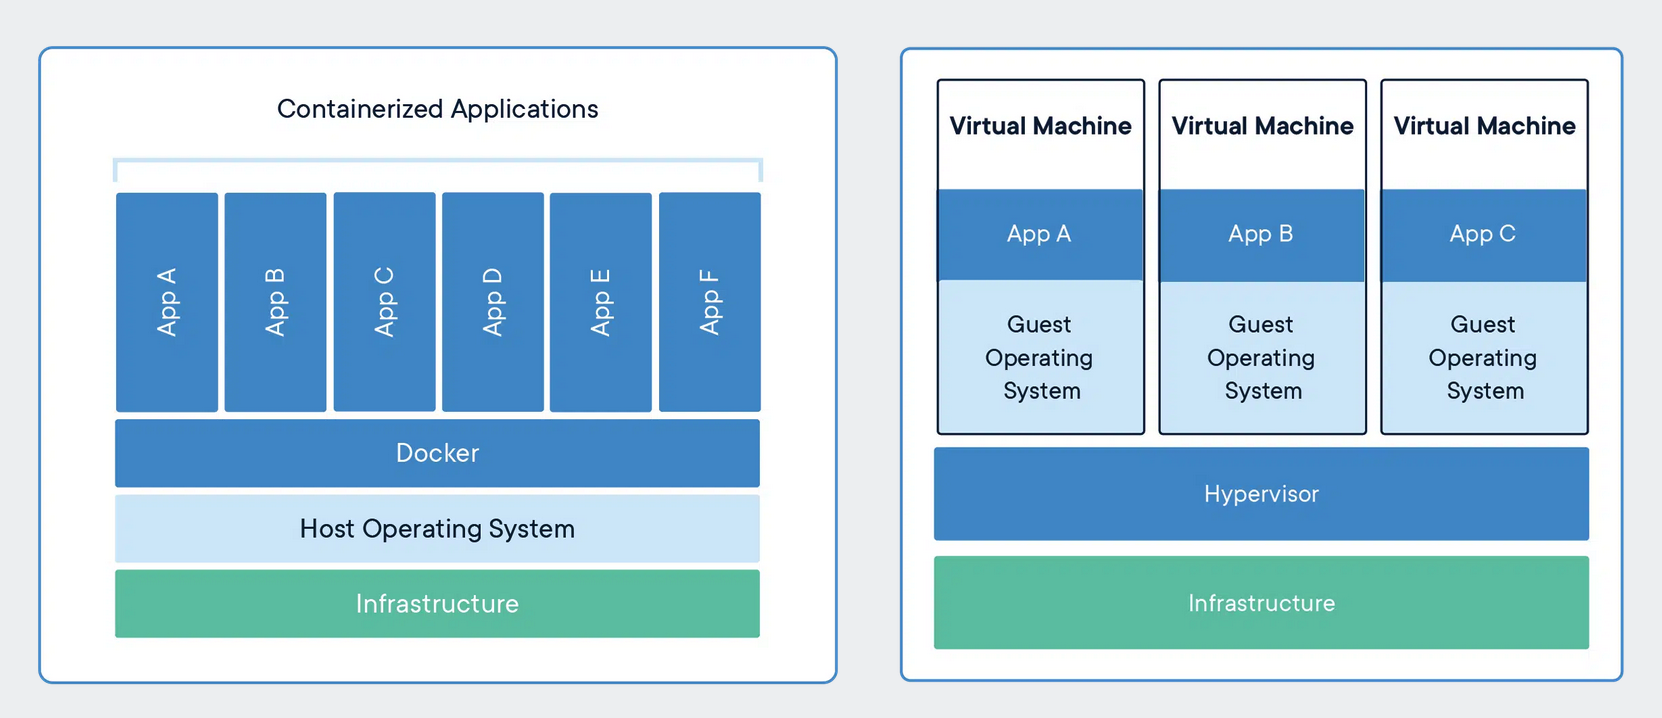
\includegraphics[width=0.95\linewidth]{DockerVsVMs.png}
\caption{\label{fig:Docker2}Docker Lifecycle.}
\end{figure}
\\
\textbf{Virtual Machines vs Docker Containers:} \\
\textbf{Virtual Machines:}
\begin{itemize}
\color{blue}
\item \textbf{Advantages}: 
\begin{itemize}
    \item isolation: VMs run separate OS, providing strict application isolation.
\end{itemize}
\item \textbf{Inefficiencies}: 
\begin{itemize}
    \item Resource Overhead: Each VM requires its OS, consuming RAM, storage and CPU. Running multiple VMs can lead to redundant resource use.
    \item Slow Boot Times: Booting a VM involves starting and entire OS, slowing down deployment.
\end{itemize}
\end{itemize}
\\
\textbf{Containers:}
\begin{itemize}
\color{blue}
\item \textbf{Efficiencies}: 
\begin{itemize}
    \item Resource Optimizations: As containers share the host OS kernel, they are exceptionally lightweight, requiring minimal RAM and storage.
    \item Rapid Deployment: Containers start almost instantaneously, accelerating both development and production.
\end{itemize}
\item \textbf{Isolation Caveats}: 
\begin{itemize}
    \item Application-Level Isolation: While Docker ensures the separation of containers from the host and other containers, it relies on the host OS for underlying resources.
\end{itemize}
\end{itemize}
%*********************************************************************
%                       Docker Lifecycle
%*********************************************************************
\newpage
\noindent
{\color{red} \rule{\linewidth}{0.5mm}}
\textcolor{red}{1. Explain the Docker lifecycle.} \\
\noindent
{\color{red} \rule{\linewidth}{0.5mm}}
There are three important things in Docker Lifecycle:
\begin{itemize}
\color{blue}
\item \textbf{docker build}: Builds docker image from Dockerfile.
\item \textbf{docker run}: runs container from docker images.
\item \textbf{docker push}: push the container image to public/private regestries to share the docker images.
\end{itemize}
\begin{figure}
\centering
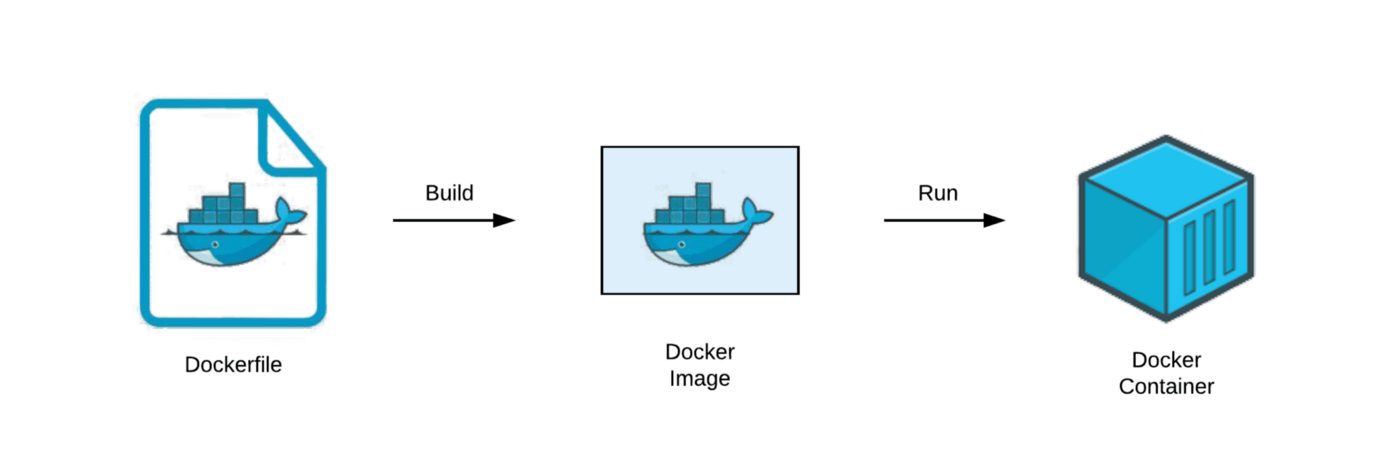
\includegraphics[width=0.95\linewidth]{Docker1.jpg}
\caption{\label{fig:Docker2}Docker Lifecycle.}
\end{figure}
%*********************************************************************
%                           Docker architecture
%*********************************************************************
\newpage
\noindent
{\color{red} \rule{\linewidth}{0.5mm}}
\textcolor{red}{1. Explain the Docker architecture.} \\
\noindent
{\color{red} \rule{\linewidth}{0.5mm}}

\begin{figure}
\centering
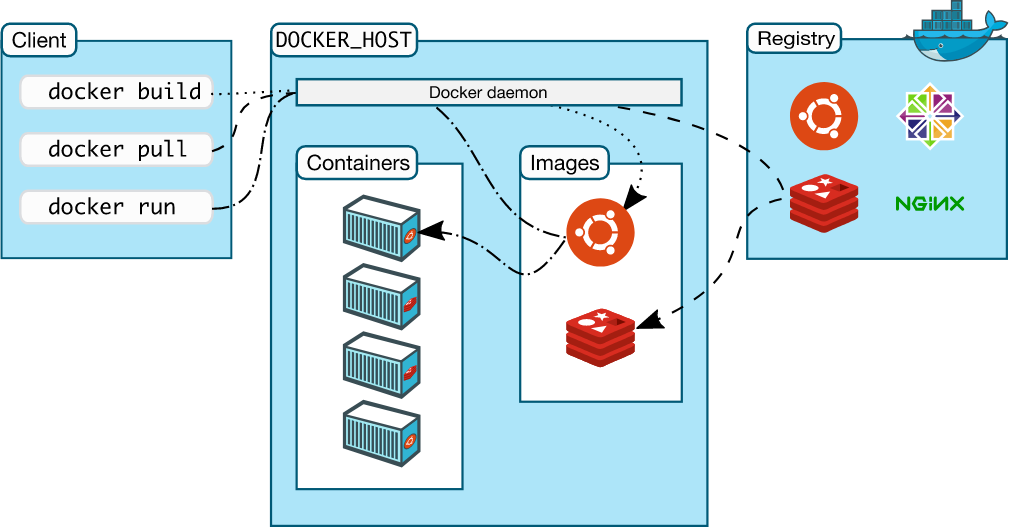
\includegraphics[width=0.95\linewidth]{DockerArchi.png}
\caption{\label{fig:Docker2}Docker Architecture.}
\end{figure}
\begin{tcolorbox}[colback=red!5!white]
    Docker Daemon is the brain of Docker.
\end{tcolorbox}
    

If Docker Daemon is killed (stops working), Docker is brain dead. \\
\textbf{Key Docker Components:} 

\begin{tcolorbox}[colback=red!5!white, colframe=red!50!black,title=Docker Daemon]
    A persistent background process that manages and executes containers. The Docker daemon (dockered) listens for Docker API requests and manages Docker objects such as images, containers, networks, and volumes. A daemon can also communicate with other daemons to manage Docker services.
\end{tcolorbox}
\begin{tcolorbox}[colback=red!5!white, colframe=red!50!black,title=Docker Client] The Docker client (docker) is the primary way that many Docker users interact with Docker. When you use commands such as docker run, the client sends these commands to dockerd, which carries them out. The docker command uses the Docker API. The Docker client can communicate with more than one daemon.
\end{tcolorbox}
\begin{tcolorbox}[colback=red!5!white, colframe=red!50!black,title=Docker Engine] 
The CLI and API for interacting with the daemon.
\end{tcolorbox}
\begin{tcolorbox}[colback=red!5!white, colframe=red!50!black,title=Docker Registry]
A repository for Docker images. Docker Hub is a public registry that anyone can use, and Docker is configured to look for images on Docker Hub by default. You can even run your own private registry.
\end{tcolorbox}


\textbf{Core Building Blocks:} 
\begin{itemize}
\color{blue}
\item \textbf{Dockerfile}: A text document containing commands that assemble container image. Dockerfile is a file where you provide the steps to build your Docker Image.
\item \textbf{Image}: A standalone, executable package containing everything required to run a piece of software. An image is a read-only template with instructions for creating a Docker container. Often, an image is absed on another image, with additional customization. For example, you may build an image which is based on the ubuntu image, but install the Apache web server and your application, as well as the configuration details needed to make your application run. \\
You might 
\item \textbf{Container}: A runtime instance of an image.
\end{itemize}

\\
\textbf{Code Example: Dockerfile} \\
\textcolor{red}{FROM} python:3.8 \\
\textcolor{red}{WORKDIR} /app\\
\textcolor{red}{COPY} requirements.txt requirements.txt\\
\textcolor{red}{RUN} pip install --no-cache-dir -r requirements.txt\\
\textcolor{red}{COPY} . .\\
\textcolor{red}{CMD} ["python", "app.py"] 
\\ 
\textbf{Core Unique Features of Docker:} \\
\begin{itemize}
\color{blue}
\item \textbf{Layered File System}: Docker images are composed of layers, each representing a set of file changes. This structure aids in minimizing image size and optimizing builds.
\item \textbf{Container Orchestration}: Technologies such as Kubernetes and Docker Swarm enable the management of clusters of containers, providing features like load balancing, scaling, and automated rollouts and rollbacks.
\item \textbf{Interoperability}: Docker containers are portable, running consistently across diverse environments. Additionally, Docker complements numerous other tools and platforms, including Jenkins for CI/CD pipelines and AWS for cloud services. 
\end{itemize}
%*********************************************************************
%               Docker Image
%*********************************************************************
\noindent
{\color{red} \rule{\linewidth}{0.5mm}}
\textcolor{red}{2. Can you explain what a Docker Image is?} \\
\noindent
{\color{red} \rule{\linewidth}{0.5mm}}
\begin{tcolorbox}[colback=red!5!white, colframe=red!50!black,title=Docker Image]
    A Docker Image is a lightweight, standalone, and executable software package that includes everything needed to run a piece of software, including the code, a runtime, libraries, environment variables, and configuration files. \\
It provides consistency across environments by ensuring that each instance of an image is identical, a key principle of Docker's build-once-run-anywhere philosophy.
\end{tcolorbox}


\textbf{Layered File System} \\
Docker images comprise multiple layers, each representing a distinct file system modification. layers are read-only, and the final container layer is read/write, which allows for efficiency and flexibility. \\   
\textbf{Key Components} \\
\begin{itemize}
\color{blue}
\item \textbf{Operating System}: Traditional images have a full or bespoke OS tailored for the application's needs. Recent developments like "distroless" images, however, focus solely on application dependencies. 
\item \textbf{Application Code}: Your code and files, which are specified during the image build.
\end{itemize}
\textbf{Image Registries} \\
Images are stored in \textbf{Docker image registries} like Docker Hub, which provides a central location for image management and sharing. You can download existing images, modify them, and upload modified versions, allowing teams to collaborate efficiently. \\
\textbf{How to build and Image?} \\
\begin{itemize}
\color{blue}
\item \textbf{Dockerfile}: Describes the steps and actions require to set up the image, from selecting the base OS to copying the application code.
\item \textbf{Build Command}: Docker's build command uses the Dockerfile as a blueprint to create the image.
\end{itemize}
\textbf{Advantages of Docker Images} \\
\begin{itemize}
\color{blue}
\item \textbf{Portability}: Docker image ensure consistent behavior across different environments, from development to production.
\item \textbf{Reproducibility}: If you are using the same image, you can expect the same application behaviour.
\item \textbf{Efficiency}: The layered filesystem reduces redundancy and accelerate deployment. 
\item \textbf{Security}: Distinct layers permit granular security control. 
\end{itemize}
\textbf{Code Example: Dockerfile} \\
Here is the Dockerfile: \\


$\#$  Use a base image \\
FROM ubuntu: latest \\

$\#$ Set the working directory \\
WORKDIR /app \\

$\#$ Copy the current directory contents into the container at /app \\
COPY ./app \\

$\#$ Specify the command to run on container start \\
CMD ["/bin/bash"]  \\



\textbf{Best practices for Dockerfiles} \\
\begin{itemize}
\color{blue}
\item Use the official base image if possible.
\item Aim for minimal layers for better efficiency.
\item Regularly update the base image to ensure security and feature updates.
\item Reduce the number of packages installed to minimize security risk.
\end{itemize}

%*********************************************************************
%                       Image vs Container
%*********************************************************************
\noindent
{\color{red} \rule{\linewidth}{0.5mm}}
\textcolor{red}{3. How does a Docker container differ from a Docker image?} \\
\noindent
{\color{red} \rule{\linewidth}{0.5mm}}
Docker images serve as templates for containers, whereas Docker containers are running instances of those images \ref{fig:Docker1}. You can run multiple containers from 1 image.   \\
\textbf{Image vs. Containers} \\
\begin{itemize}
\color{blue}
\item \textbf{Image}: A static package that encompasses everything the application requires to run.
\item \textbf{Container}: An operating instance of an image, running as a process on the host machine.
\end{itemize}
\textbf{Key Distinctions}
\begin{itemize}
\color{blue}
\item \textbf{State}: Containers encapsulate both the application code and its runtime environment in a stable and consistent state. In contrast, images are passive and don't change once created.
\item \textbf{Mutable vs Immutable}: Containers like any running process, can modify their state. In contrast, images are immutable and do not change once built.
\item \textbf{Disk Usage}: Containers have both writable layers (such as logs or configuration files) and read-only layers (the image layers), potentially leading to increased disk usage over time. Docker's use of layered storage, however, limits this growth. Images, on the other hand, are solely read-only, meaning each instance based on the same image doesn't consume additional disk space. 
\end{itemize}



\begin{figure}
\centering
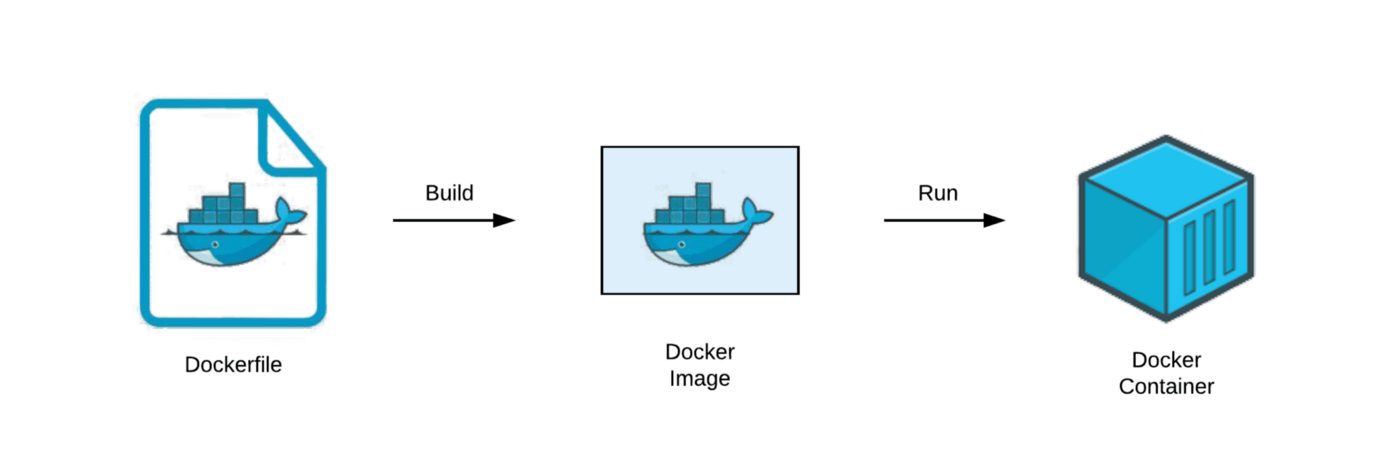
\includegraphics[width=0.95\linewidth]{Docker1.jpg}
\caption{\label{fig:Docker1}TDocker File to Container.}
\end{figure}

\textbf{Practical Demonstration} \\
Here is the code:
\begin{enumerate}
    \item \textbf{Dockerfile} - Define the image:
    \item \textbf{Building an Image} - Use the 'Docker build' command to create the image.
    \item \textbf{Instantiating Containers} - Run the built image with 'docker run' to spawn a container.
    \item \textbf{Viewing Containers} - The 'docker container ls' or 'docker ps' commands display active containers.
    \item \textbf{Modifying Containers} - As an example, you can change the content of a container by entering in via 'docker exec'. \\
    docker exec -it mycontainer /bin/bash
    \item \textbf{Stopping and Removing Containers} - This can be done using the 'docker stop' and 'docker rm' commands otr combined with the '-f' flag. \\
    docker stop mycontainer \\
    docker rm mycontainer 
    \item \textbf{Cleaning up Images} - Remove any unused images to save storage space. \\
    docker image prune -a
\end{enumerate}


%*********************************************************************
%       Docker Hub and Use
%*********************************************************************
\noindent
{\color{red} \rule{\linewidth}{0.5mm}}
\textcolor{red}{4. What is the Docker Hub and what is it used for?} \\
\noindent
{\color{red} \rule{\linewidth}{0.5mm}}
The Docker Hub is a public cloud-based registry for Docker images. It's a central hub where you can find, manage, and share your Docker container images. Essentially, it is a version control system for Docker containers. \\
\textbf{Key Functions}
\begin{itemize}
    \item \textbf{Image Storage}
    \item \textbf{Versioning}
    \item \textbf{Collaboration}
    \item \textbf{Link to GitHUb}
    \item \textbf{Automation}
    \item \textbf{Webhooks}
    \item \textbf{Security Scanning}
\end{itemize}
%*********************************************************************
%                   Dockerfiles
%*********************************************************************

\noindent
{\color{red} \rule{\linewidth}{0.5mm}}
\textcolor{red}{5. Explain the Dockerfile and its significance in Docker.} \\
\noindent
{\color{red} \rule{\linewidth}{0.5mm}}
One of the defining feature of Docker is its use of Dockerfiles to automate the creation of container images. A Dockerfile is a text document that contains all the commands a user could call on the command line to assemble an image. \\
\textbf{Common Commands}:
\begin{itemize}
    \item \textbf{\textcolor{Red}{FROM}}: \textcolor{PineGreen}{Sets the base image for subsequent build stages}
    \item \textbf{\textcolor{Red}{RUN}}: \textcolor{PineGreen}{Executes commands within the image and then commits the changes}
    \item \textbf{\textcolor{Red}{EXPOSE}}: \textcolor{PineGreen}{Informs Docker that container listens on specific port.}
    \item \textbf{\textcolor{Red}{ENV}}: \textcolor{PineGreen}{Sets environemnt variables.}
    \item \textbf{\textcolor{Red}{ADD/COPY}}: \textcolor{PineGreen}{Adds files from the build context into the image.}
    \item \textbf{\textcolor{Red}{CMD/ENTRYPOINT}}: \textcolor{PineGreen}{Specifies what command to run when the container starts. }
\end{itemize}
\\
\textbf{Multi-Stage Builds}:
\begin{itemize}
    \item \textbf{\textcolor{Red}{FROM}}: \textcolor{PineGreen}{Allows for multiple build stages in a single Dockerfile.}
    \item \textbf{\textcolor{Red}{COPY}}: \textcolor{PineGreen}{Enables copying from another build stage, useful for extracting build artifacts. }
\end{itemize}
\textbf{Image Caching}:
Docker uses caching to speed up build processes. If a layer changes, Docker rebuilds it and all those that depend on it. Often, this results in fortuitous cache misses, making builds slower than anticipated. \\
To optimize, place commands that change frequently (such as file copying or package installation) toward the end of the file. \\
Docker Build Accesses a remote repository, the Docker Cloud. The build context is the absolute path or URL to the directory containing the Dockerfile. 
\\
\textbf{Tips for Writing Efficient Dockerfiles}
\begin{itemize}
    \item \textbf{Use Specific Base Images}: Strat from the most lightweight, appropriate image to keep your build lean.
    \item \textbf{Combine Commands}: Chaining commands with $\&\&$ (where viable) reduces layer count, enhancing efficiency. 
    \item \textbf{Remove Unneeded Files}: Eliminates files your application doesn't require, especially temporary build files or cached resources.
\end{itemize}
\textbf{Code Example: Dockerfile for a Node.js Web Server}:
\begin{itemize}
    \item \textbf{\textcolor{Red}{FROM}}: \textcolor{PineGreen}{node:14-alpine} $\#$ Use a specific version of Node.js as the base.
    \item \textbf{\textcolor{Red}{WORKDIR}}: \textcolor{PineGreen}{/app} $\#$ Set the working directory in the container. 
    \item \textbf{\textcolor{Red}{COPY}}: \textcolor{PineGreen}{package*.json ./} $\#$ Copy pacakge.json and package-lock.json first to leverage caching when the dependencies haven't changed. 
    \item \textbf{\textcolor{Red}{RUN}}: \textcolor{PineGreen}{npm install --only=production} $\#$ Install NPM dependencies.
    \item \textbf{\textcolor{Red}{COPY}}: \textcolor{PineGreen}{ . .} $\#$ Copy the rest of teh application files.
    \item \textbf{\textcolor{Red}{EXPOSE}}: \textcolor{PineGreen}{3000} $\#$ Expose port 3000
    \item \textbf{\textcolor{Red}{CMD}}: \textcolor{Blue}{["node", "app.js"]} $\#$ Start the Node.js application.
\end{itemize}
\\
%*********************************************************************
%                       Layer
%*********************************************************************
\noindent
{\color{red} \rule{\linewidth}{0.5mm}}
\textcolor{red}{6. How does Docker use layer to build images?} \\
\noindent
{\color{red} \rule{\linewidth}{0.5mm}}


Docker allows a Layered File System approach, employing Union File System like AUFS, OverlayFD, and DeviceMapper to stack image layers. \\
This structure enhances modularity, storage efficiency, and image-building speed. It also offers read-only layers for image consistency and integrity. 
\\
\textbf{Union File Systems} \\
Union File Systems permit stacking multiple directories or file systems, presenting them coherently as a single unit. While several such systems  are in use, AUFS and OverlayFS are notably popular. 
\begin{itemize}
    \item \textbf{AUFS}: A front-runner for a long time, AUFS offers versatile compatibility but is not part of the Linux kernel. 
    \item \textbf{OverlayFS}: Now integrated into the Linux kernel, OverlayFS is lightweight and provides backward compatibility with ext4 and XFS. 
\end{itemize}
\textbf{Image Layering in Docker} \\
When stacking Docker image layers, it's akin to a file system with read-only layers superimposed by a writable layer, the container layer. This setup ensures separation and persistence:
\begin{itemize}
    \item \textbf{Base Image Layer}: This is the foundation, often comprising the operating system and core utilities. It's mostly read-only to safeguard uniformity.
    \item \textbf{Intermediate Layers}: These are interchangeable and encapsulate discrete modifications. Consequently, they are also mostly read-only.
    \item \textbf{Topmost or Container Layer}: This layer records real-time alterations made within the container and is mutable. 
\end{itemize}
\textbf{Code Overlayers} \\
Here is the code:
\begin{enumerate}
    \item Each layer is defined by Dockerfile instruction.
    \item The base image is ubuntu:latest, and the application code is stored in a file named app.py
\end{enumerate}
\begin{itemize}
    \item \textbf{\textcolor{Red}{FROM}}: \textcolor{PineGreen}{ubuntu:latest} $\#$ Start from base image.
    \item \textbf{\textcolor{Red}{WORKDIR}}: \textcolor{PineGreen}{ /app} $\#$ Set the working directory in the container. 
    \item \textbf{\textcolor{Red}{COPY}}: \textcolor{PineGreen}{app.py /app} $\#$ Copy the application code
    \item $\#$ Placeholder for Dockerfile \\ $\#$ ... 
\end{itemize}
%*********************************************************************
%                           COPY and ADD Difference
%*********************************************************************
\noindent
{\color{red} \rule{\linewidth}{0.5mm}}
\textcolor{red}{7. What is the difference between the COPY and ADD commands in a Dockerfile?} \\
\noindent
{\color{red} \rule{\linewidth}{0.5mm}}
\textbf{Purpose} \\
\begin{itemize}
    \item \textbf{COPY} - Designed for straightforward files and directory copying. It's the preferred choice for most use-cases. 
    \item \textbf{ADD} - Offers additional features such as URI support. However,since it is more powerful, it is often recommended to stick with COPY unless you specifically need the extra capabilities. 
\end{itemize}

%*********************************************************************
%*********************************************************************
\noindent
{\color{red} \rule{\linewidth}{0.5mm}}
\textcolor{red}{8. What is the purpose of the .dockerignore file?} \\
\noindent
{\color{red} \rule{\linewidth}{0.5mm}}

%*********************************************************************
%*********************************************************************
\noindent
{\color{red} \rule{\linewidth}{0.5mm}}
\textcolor{red}{9. How would you go about creating a Docker image from and exiting container?} \\
\noindent
{\color{red} \rule{\linewidth}{0.5mm}}

%*********************************************************************
%*********************************************************************
\noindent
{\color{red} \rule{\linewidth}{0.5mm}}
\textcolor{red}{10. In practice, how do you reduce the size of Docker images?} \\
\noindent
{\color{red} \rule{\linewidth}{0.5mm}}


%*********************************************************************
%*********************************************************************
\noindent
{\color{red} \rule{\linewidth}{0.5mm}}
\textcolor{red}{11. What command is used to run a Docker container from an image?} \\
\noindent
{\color{red} \rule{\linewidth}{0.5mm}}

%*********************************************************************
%*********************************************************************
\noindent
{\color{red} \rule{\linewidth}{0.5mm}}
\textcolor{red}{12. Can you explain what a Docker namespace is and its benefits?} \\
\noindent
{\color{red} \rule{\linewidth}{0.5mm}}


%*********************************************************************
%*********************************************************************
\noindent
{\color{red} \rule{\linewidth}{0.5mm}}
\textcolor{red}{13. What is the Docker volume and when would you use it?} \\
\noindent
{\color{red} \rule{\linewidth}{0.5mm}}


%*********************************************************************
%*********************************************************************
\noindent
{\color{red} \rule{\linewidth}{0.5mm}}
\textcolor{red}{14. Explain the use and significance of Docker-compose tool.} \\
\noindent
{\color{red} \rule{\linewidth}{0.5mm}}

%*********************************************************************
%*********************************************************************
\noindent
{\color{red} \rule{\linewidth}{0.5mm}}
\textcolor{red}{Definitions} \\
\noindent
{\color{red} \rule{\linewidth}{0.5mm}}

\begin{tcolorbox}[colback=red!5!white, colframe=red!50!black,title=Port Binding:] Bind the container's port to the host port to make the service available to the outside world. Nginx runs on port 80, Reddis on port 6379. 
\end{tcolorbox}

\begin{tcolorbox}[colback=red!5!white, colframe=red!50!black,title=Commands] 
\begin{itemize}
    \item \textbf{docker images}: Shows all images that we have locally.
    \item \textbf{docker images | grep python}
    \item \textbf{docker pull \{name\}:\{tag\} }: Pull an image from a registry. docker pull nginx:1.23. Docker client will contact Docker Hub to grab nginx with 1.23 tag and download it locally. It pulls the image from the image registry- docker hub. 
    \item Docker Hub registry (docker.io) is used by default. 
    \item Now that we have images locally. They are only useful when we \textbf{run an image in the container environment}. We pick the image that we have locally with the tag and run the docker run command.
    \item \textbf{docker run}: Creates a new container every time. It does not reuse the container that we created previously.
    \item \textbf{docker run \{name\}:\{tag\} } Creates a container from a given image and starts it. \textbf{docker run nginx:1.23}. Starts the container based on the image. We can see that the logs on nginx service start up inside the container. \textit{Docker generates a random name for the container automatically if you do not specify it}.
    \item \textbf{-d or --detach}: flag- Start a container in the background without blocking the terminal . Runs container in the background and prints the container ID. \textbf{docker run -d nginx:1.23}
    \item \textbf{-p}: flag- .
    \item \textbf{--name}: flag- assign a name to the container.
    \item \textbf{docker --name web-app -d -p 9000:80 nginx:1.23}
    \item \textbf{docker ps}: List the running containers. It does not show the ones that were created and stopped.
    \item \textbf{docker logs web-app}
    \item \textbf{docker ps (flag)-a or --all}: List all containers (stopped and running). 
    \item \textbf{docker stop \{containerID\ \{containerName\}}: Stop one or more active containers.
    \item \textbf{docker start \{containerID\} \{containerName\}}: Start one or more inactive but existing containers.
    \item \textbf{-p or --publish}: Publish a container's port to the host.
    \item \textbf{-p \{HOST\_PORT\}:\{CONTAINER\_PORT\} }
    \item \textbf{docker run -d -p 9000:80 nginx:1.23}: Only 1 service can run on a specific port of the host. e.g. Only 1 service can run on port 9000
    \item \textbf{localhost:9000}: on the browser.
    \item \textbf{docker logs \{containerID\} }
    \item Choosing host port: Standard to use same port on host machine as the container is using.
\end{itemize}
\end{tcolorbox}

%*********************************************************************
%*********************************************************************
%*********************************************************************
%*********************************************************************
\noindent
{\color{red} \rule{\linewidth}{0.5mm}}
\textcolor{red}{15. Can Docker containers running on the same host communicate with each other by default? If so, how?} \\
\noindent
{\color{red} \rule{\linewidth}{0.5mm}}
\section{Reference}
\begin{itemize}
    \item \href{https://github.com/Devinterview-io/docker-interview-questions}{DockerQ\&A}
    \item \href{https://labs.iximiuz.com/tutorials/docker-container-management-commands}{Main Docker Commands}
    \item \href{https://github.com/iam-veeramalla/Docker-Zero-to-Hero}{Docker Tutorial}
\end{itemize}
\end{document}